\documentclass[a4paper,10pt]{article}
\usepackage[utf8]{inputenc}


% For the \todo{} command.
\usepackage{todo}

% Nice fonts
\usepackage{palatino}
% For doubled lines in tables.
% Useful for separation of table header from table body.
\usepackage{hhline}
\usepackage[english]{babel}
\usepackage{tabularx}
% Needed for Listings package with Eiffel.
% \usepackage{xcolor}
% Source code listings.
\usepackage{listings}
% Appendix with extra title.
% \usepackage [page] {appendix}
% To include PNG files.
\usepackage{graphicx}
% Nice looking captions.
\usepackage[font={footnotesize,sl}, labelfont=bf] {caption}
% Include PDF pages.
% \usepackage{pdfpages}

% Clickable links. Has to be the last package:
\usepackage [hidelinks] {hyperref}


\lstset{language=C,basicstyle=\ttfamily\small}


\newcommand{\todoref}{\todo{ref}}
\newcommand{\filepath}[1]{\emph{ #1}}

% Title Page
\title{Advanced Operating Systems \\ Project Report}
\author{Roman Schmocker \\ Yauhen Klimiankou}


\begin{document}

\maketitle


\section{Introduction}

This report provides documentation for the operating system which we built as part of the project in the Advanced Operating Systems course.
The code is based on a stripped-down version of Barrelfish \cite {web:barrelfish}.

\todo{ more introduction}

\section{Getting started}

\begin{lstlisting}

void test_listings_package (void);

void test_listings_package (void)
{
  uint32_t an_int;
  char* a_string = "asdf";
  for (int i=0; i<42; i++) {
    printf (a_string);
  }
}
\end{lstlisting}


\section {Modules}

\subsection{Paging}

% 
% - Intent: quick lookup of page table, ``unmap'' requests from memory server
% 
% - Data structues
% -- Simple for virtual memory
% -- 2-level array for page tables (mirroring actual page tables)
% -- linked list for frames
% 
% - Problem: No unmap from domain itself
% -- esp. no recycling of virtual addresses
% -- we thought that malloc would never return memory anyway
% -- didn't think about domain spawning / bulk transfer with explicit map/unmap operations

The paging code is mostly contained in \filepath{lib/barrelfish/paging.c} and the corresponding header file.
The central element is the \lstinline!paging_state! struct.
When desgining the data structure for the paging code we wanted to support the following functions in constant time:

\begin{itemize}
 \item Check if an address is valid.
 \item Lookup of the page tables associated to the virtual address.
 \item Allocation of a physical frame for a page.
 \item Deallocation of a frame when the memory server asks for it.
\end{itemize}

To support the first use case we just keep track of the allocated range of virtual addresses using two integer variables.
That way determining if a page fault is ``valid'' is very simple: 
If it's in the range, everything is ok and we can map the page to a frame, and if not we abort due to an invalid address.

The data structure of choice to represent the page table structure is a two-level array that mirrors the actual page tables in memory.
Currently we only store the capability to the page tables and whether a certain page has been allocated at some point.
We don't yet store any flags, pointers to a swap file or other metadata, but it would be easy to add this information.

Frame management is a bit more complex because we always allocate frames of 1 MiB.
That way we can avoid an IPC call for every single page fault, but we also have to keep track of free and allocated space within a frame.
The \lstinline!struct frame_list! manages this information for a single frame.
To support the last use case it also keeps track of the actual pages stored on this frame.
The \lstinline!paging_state! struct then maintains a double ended queue of \lstinline!frame_list! nodes, where only the frame at the head of the list may contain some free space.

As already mentioned, an important use case we had in mind were requests to return a frame from the memory server.
We never implemented that functionality, but the data structure is designed to support it.
An implementation would have to do the following:
\begin{itemize}
 \item Remove the last \lstinline!frame_list! element.
 \item Write all pages backed by this frame to disk.
 \item (Optionally) update some flags and metadata in the page table array.
 \item Return the frame to the memory server.
\end{itemize}

The data structures used to track frames and page tables need some form of dynamic memory management.
Unfortunately however we can't use malloc/free in our paging implementation, because this memory is not initially mapped.
Therefore we used slab allocators (from \filepath{include/barrelfish/slab.h}) to manage the memory needed by these data structures.
The feature \lstinline!memory_refill! in our paging code is used to enlarge the pool of usable memory if the slab allocators run out of space.

\subsubsection{Assessment}

Our initial design of the paging module turned out to be rather flexible.
Over the course of the project, we only had to change small things, like adding another slab allocator for exception stacks of user-level threads 
or implementing \lstinline!paging_map_fixed_attr!, where we could adapt an existing function that did almost the same job.

The only thing that proved to be insufficient was the management of virtual address space.
The initial assumption that only malloc/free can issue unmap operations (and never does as it's not implemented) was wrong.
There are some parts in the code that directly interacts with the paging library and needs to ``free'' a range of virtual memory sometimes, among them the spawndomain library or the bulk transfer mechanism.

Supporting this would have required us to rewrite a lot of existing code, and that's why we didn't do it in the end.
This in turn means that our current solution leaks virtual addresses, but we tried to reduce this as much as possible by reusing the ranges of virtual memory.

\subsection{Local Message Passing}

The local message passing (LMP) system is mostly implemented in \filepath{lib/barrelfish/aos\_rpc.c} for the client side.
Some generic server-side features are implemented in \filepath{lib/aos\_support/server.c}.

The LMP system has some important characteristics:
\begin{itemize}
 \item All messages are synchronous, i.e. receive is blocking.
 \item The channels are always one-to-one connections.
 \item The communication is client-server style.
 \item We support direct connections to any server (i.e. no indirection through init).
 \item Every ``send'' message has an enum constant as its first argument that denotes the message type.
 \item Every ``reply'' message has an error code as its first argument.
 \item All other arguments are determined by the actual message type.
\end{itemize}

The individual message types and their arguments are described in the header file \filepath{include/barrelfish/aos\_rpc.h}.
To support writing code on the client side we implemented the feature \lstinline!aos_send_receive! which takes a struct containing all arguments, 
sends a request to the server, waits for a reply, and copies the receive arguments back into the struct.
That way we could avoid some code duplication for every remote procedure call.

Some servers provide core system services. Init for example provides RAM, and the serial\_driver provides I/O.
We therefore provide some predefined channels to these services which are initialized in \filepath{lib/barrelfish/init.c}.
The channels can be retrieved with the functions \lstinline!aos_rpc_get_init_channel! and \lstinline!aos_rpc_get_serial_driver_channel!, respectively.

\subsubsection{Connection setup and name service}

In our LMP implementation we wanted to support direct channels between two domains.
To do that we had to implement some additional functionality, in particular a simple name service and a mechanism to set up a new connection.

The design of the name service is very simple.
In \filepath{aos\_rpc.h} we added an enum type \lstinline!aos_service! which is used for some of the core system services, such as the serial driver or the FAT file system.
Each domain that acts as a server for such a core system service then has to register itself via the \lstinline!AOS_RPC_REGISTER_SERVICE! LMP message.
Init itself keeps track of all registered servers and therefore acts as a name service.

When a client wants to find a particular service, it sends a request to init, and init replies with a new endpoint capability of the specified domain.
This was a bit tricky to implement, because we only allow one-to-one connections, so init first has to request a new endpoint from the (registered) server.
Init shouldn't mix the reply however with some other request from another domain, therefore we had to break our usual send-reply protocol and plan this interaction carefully.

In chronological order, this is what happens when a domain wants to find, for example, the serial driver:

\begin{itemize}
 \item The client sends an \lstinline!AOS_RPC_FIND_SERVICE! with the enum constant of the serial driver to init.
 \item Init uses a new request ID (a ``cookie'') and remembers the channel that sent the request.
 \item Init checks if the serial driver is registered and sends an \lstinline!AOS_ROUTE_REQUEST_EP!.
 This call includes the previously generated request ID.
 \item The serial driver handles the enpoint request call by creating a new channel.
 It replies to init with an \lstinline!AOS_ROUTE_DELIVER_EP! which contains the new endpoint and the unchanged request ID as arguments.
 Note that this RPC call doesn't follow the usual send-reply style message exchange, because the reply contains a message type argument.
 \item Thanks to the special reply format init can handle the request like any other LMP message.
 When receiving the \lstinline!AOS_ROUTE_DELIVER_EP!, init retrieves the channel that initially sent the \lstinline!AOS_RPC_FIND_SERVICE! request using the request ID and forwards the endpoint.
 \item The client domain wakes up again receives the new endpoint, which it can then use to establish a direct connection to the serial driver.
\end{itemize}


% - Synchronous message passing, one-to-one
% - channels between any client/server possible (not just init)
% - general format: service identifier, args -> reply: error code, args
% - aos\_rpc.c: client API
% -- support feature \lstinline!aos_send_receive!
% -- only initialize arguments and receive result.
% - aos\_support/server.c: generic server support routines
% - routing: in init - service registration, find requests
% - bulk transfer: shared buffer, bound to a channel
% - predefined channels (provided by libbarrelfish): init, serial\_driver


\subsubsection{Bulk transfer}

For a long time throughout the project we only had the basic message-passing communication model.
Although this worked well, we always had to split an IPC call into several messages if the data to be transmitted exceeded the capacity of a single message.
This was a tedious and error prone process, and due to this we decided to add a mechanism for bulk transfer.

The basic idea is to set up a buffer which is shared between client and server.
This setup is initiated by the client, and only when it is actually needed.

We added a new message type which allowed a client to share a frame with a buffer and get back a \lstinline!memory_descriptor!, which it can use afterwards for other IPC calls.
The server-side part is implemented in \filepath{lib/aos\_support/}, which had the nice side effect that every server gained the buffer sharing mechanism for free without any further changes.
The client-side part is implemented in \filepath{lib/barrelfish/aos\_rpc.c}, where it is now possible to ``attach'' a shared buffer to any \lstinline!struct aos_rpc! channel.

The bulk transfer mechanism was a pretty late addition to the code base, therefore not all RPC calls have been changed to make use of it yet.

\subsection{Shell}
	Shell is a standard mean of communication and interaction between user and developed operating system.
	In the same time it is the only user interface currently existing in OS.
	 
	Historically shell was grew up in the context of memeater module and in some moment almost completely preempt its original functionality. The source code can be find at path \filepath{usr/memeater/memeater.c}.
	
	The main difference of the our shell from the conventional shells is that in fact it is remote shell which uses the host system as an source of input and target for output streams. 
	Communication with the host computer system goes through serial port interface (also knows as RS-232) for which incoming stream of characters is treated as a standard input stream and outgoing set of characters is treated as a standard output stream in terms of C language. 
	Host computer system is such design plays o role of conventional terminal by connecting the input stream stream of characters from the serial port with display and pushing the characters inputted from keyboard to the same serial port.
	Picocom utility is in use for maintaining of this bridge on the host Linux-based host.
	
	Communication via serial port is implemented in separate server called serial driver., located at path \filepath{usr/serial\_driver/}.
	Shell interacts with this driver using functions from the set of standard IO library of C and AOS RPC calls \lstinline!aos_rpc_serial_getchar! and \lstinline!aos_rpc_serial_putchar!.
	
	Like most of the servers execution of the server consist of three phases:
	\begin{enumerate}
		\item Initialization.
		\item Service loop.
		\item Deinitialization.
	\end{enumerate}
	During the initialization phase shell sets up its global state and establishes connections with other system components which will be used in the service loop.
	The set of system components used by shell includes:
	\begin{enumerate}
		\item Filesystem driver.
		\item Led driver.
		\item Process manager.
		\item Serial diver.
	\end{enumerate}
	Global state of the shell consist of:
	\begin{enumerate}
		\item Sign of termination.
		\item String describing the current directory.
	\end{enumerate}
	
	Service loop of the shell is conditionally endless loop which is run until the sign of termination will not be set. 
	Each iteration of this loop handles one input request an d consist of several steps:
	\begin{enumerate}
		\item Assembling of the request string.
		\item Splitting of the assembled request into two parts: command and arguments.
		\item Look up of the executor.
		\item Execution of the request.
	\end{enumerate} 
	Purpose of the first step is to split endless input stream coming from the serial port via serial driver into separate strings each of which represent single request (implemented in function \lstinline!receive_request!).
	Carriage return character of ASCII encoding table is used as a separator between sequential requests.
	Function \lstinline!receive_request! also reflects each incoming character back to the serial port.
	This reflection allows user on the host see what he types on keyboard in real time and by this control correctness of input and reply for the inputted request from the shell running on Pandaboard.
	Unfortunately, Picocom doesn't support the special handling of the control characters and by default displays all characters disregard to its nature.
	As a result typo in the inputting command can be fixed only by flushing the current wrong request and retyping it again.
	Once the complete request is assembled it is passed to the second step of service loop iteration.
	  
	To facilitate request processing it splits into two parts -- command and arguments.
	Command is considered as a first word of request where arguments is a rest of the request.
	Space characters between command and arguments are omitted.
	At the current state shell doesn't make splitting of the arguments string into separate argument words.
	Instead, it is responsibility of each command executor to split and process arguments in appropriate way. 
	
	  Shell support two types of commands:
	  \begin{enumerate}
	  	\item Internal
	  	\item External
	  \end{enumerate}  
	  Internal commands implementations are embedded into the shell itself. List of internal commands can be found in table \ref{tbl:icl}.
	  External commands are expected to be implemented as a separate processes and shell expect that appropriate binaries are part of the Barrelfish boot image.
	  Internal commands have a priority over external commands.
	  As a result, there is no way to execute external command with the same name as one of the internal commands have.
	  Internal commands look up implemented as a simple loop through the internal command table until entry with the same name won't be found. 
	  
	\begin{table}[h]
       		\centering
        	\begin{tabular}{| m{2.0cm} | m{1.5cm} | m{7.0cm} |}
			\hhline{===}
            		\textbf{Command name} 	& \textbf{Args} 	& \textbf{Description}	\\
			\hhline{===}
            		cat 				& file path 							& Display the content of a file specified as an argument. 																\\ \hline
            		cd 				& --- \newline file path \newline \newline	& Sets the current directory to root \newline	Set the current directory in accordance with absolute or relative path specified in the argument	.	\\ \hline
            		echo 				& string 							& Display a string specified as an argument																			\\ \hline
            		exit 				& --- 							& Force termination of shell																						\\ \hline
            		kill 				& integer 							& Force termination of the process which PID specified as an argument. Init process (PID 0) can't be terminated.						\\ \hline
            		ledoff			& ---								& Turn off the led on the Pandaboard.																				\\ \hline
            		ledon				& --- 							& Turn on the led on the Pandaboard.																				\\ \hline
            		ls 				& --- 							& Display list of files and directories from the current directory.															\\ \hline
            		oncore			& integer + string 					& Execute request specified as a string on kernel which id specified as an integer. Can be used to execute programs on slave kernel.			\\ \hline
            		ping 				& --- 							& Send series of `Ping' messages to the `test\_domain' process. Expects that last one in the running state.							\\ \hline
            		ps 				& --- 							& Display the currently-running processes.																			\\ \hline
            		run\_memtest		& integer 							& Run memory allocation test, which allocates and fills memory chunk of specified size. 											\\ \hline
            		test\_string		& --- 							& Send very long predefined string to the serial driver and by this display it.													\\ \hline            		
        	\end{tabular}
        	\caption{List of shell internal commands}
        	\label{tbl:icl}
	\end{table}
	
	External commands can be executed in two modes: background and foreground.
	By default shell execute commands on the foreground mode, but execution of the command in the background mode can be forced by putting the `\&' character at the end of request.
	Command running in the foreground mode suspends the shell until command executor process will be terminated and intercepts control over serial port channel.
	Command running in background mode runs concurrently with the shell and without access to the serial port channel.
    	    	
	 \subsection{Serial I/O}
	 	The serial driver is a mediator between serial port connection and the rest of the rest of operating system. It is located in \filepath{usr/serial\_driver/}.
	 	It have straightforward implementation due to the simplicity of the serial port management at least on the level of use which we have.
	 	Driver didn't support buffering, interrupts, baud rate control etc. and relies to the preliminary port serial port initialization made by kernel during boot up.
	 	
	 	Handling of the serial port is is based on polling.
		
		Driver provides the next set of services:
		\begin{enumerate}
			\item Put char. Output character into serial port.
			\item Get char. Input character from the serial port.
			\item Put string. Output a string of characters to the serial port. This makes use of the bulk transfer mechanism to avoid splitting and transmitting the string in small chunks.
			\item Set foreground. Set the process id of the process which will be the only process eligible to receive input from the serial port.
		\end{enumerate}
		
		In addition for convenience the libc was customized to use serial port driver as back end for the prinf and scanf families of functions.
		As a result any application is able to use traditional C-like IO.

\subsection{Process management}
\label{sec:process-management}

Spawning and managing domains is done in init.
The relevant code can be found in \filepath{usr/init/process\_manager.c}, \filepath{usr/init/main.c} and \filepath{lib/aos\_support/module\_manager.c}.
The latter keeps track of the modules shipped with the multiboot image and maps them into init's address space.

The process manager is responsible to spawn a new domain and keep track of all running domains.
The main data structure within the process manager is the \lstinline!domain_info! struct.
It keeps track of a domain's state, its dispatcher and CSpace, and its channel to \emph{init}.

The most important function is \lstinline!spawn!, which takes the name of a domain as an argument.
The function does all the steps required to spawn a new domain:
\begin{itemize}
 \item Loading the multiboot module.
 \item Setting up the Dispatcher, CSpace and VSpace.
 \item Parse and relocate the ELF image.
 \item Create the channel between init and the new domain.
 \item Store relevant data in the \lstinline!domain_info! struct.
 \item Make the domain runnable.
\end{itemize}

The process manager maintains an array of \lstinline!domain_info! structs to keep track of all spawned domains.
The array index serves as a unique domain identifier.
If the initial length of the array is insufficient it can be dynamically grown, so we don't have a hard limit on the number of possible domains.
The \lstinline!ps! command dumps the name and domain ID of every domain stored within the array.

\subsubsection {Domain Teardown}

Tearing down a domain is challenging in barrelfish.
The first issue we had to solve is to realize \emph{when} a domain needs to be cleaned up, i.e. we needed to get some notification that a domain has stopped running.
To solve this problem we added a new IPC call \lstinline!AOS_RPC_KILL! which can be used to kill a domain, given a domain ID.
We then adapted \lstinline!libc_exit! in \filepath{lib/barrelfish/init.c} to perform this call with its own ID (i.e. the domain commits suicide).

Init therefore gets a notification that some domain wants to be killed.
It can then revoke the dispatcher capability to make the domain unrunnable.

The next step would be to properly clean up the domain.
This would consist of returning all frames and device frames to the corresponding server and revoke the root CNode to clean up the capability space.
We could only implement the last part however, as keeping track of allocated frames for each domain would have required us to do some major refactoring.
This in turn means that we're leaking memory for each spawned domain, and it's the reason why a domain never leaves the \emph{zombie} state as for now.

The introduction of \lstinline!AOS_RPC_KILL! allowed us to introduce another mechanism.
A domain can now issue an \lstinline!AOS_RPC_WAIT_FOR_TERMINATION! to get a notification as soon as another domain stops.
The shell makes use of this facility to suspend itself during foreground tasks.
And because we already had the \lstinline!AOS_RPC_KILL! call we could also very easily extend our shell to spawn process in the background and \emph{kill} them later.

\subsubsection{Assessment}
Our domain management code went through many refactorings, and we're still not quite happy.
The main problem is to properly clean up a zombie domain.

It would be necessary to keep track of frames and device frames allocated by that domain and return them to the servers upon teardown.
This would have meant to introduce a lot more state and changes in existing IPC calls to keep track of allocated frames.
A potential problem is the bulk transfer mechanism, where frames are shared between client and server, and it might not be that easy to revoke these frames.
With some more time we may have been able to find a solution, but it's certainly not an easy task.

% - currently done in init
% - server manages process table and info about loaded modules
% -- can be printed with ps command
% - shell attempts to start program with specific name if command not recognized
% - mechanism to register for end notification (foreground tasks)
% - kill command to revoke dispatcher capability (background tasks)
% - no further cleanup for zombie domains as for now

\subsection{Mupltiple Cores}

\subsubsection{Preparing the kernel image}

The preparation of the kernel image is mostly done in \filepath{usr/init/cross\_core\_setup.c}.
The implementation is heavily inspired\footnote{copy-pasted} from the upstream Barrelfish code base.
Compared to the upstream mechanism we implemented some simplifications however, since we don't have to support more than two cores.
We also adapted the code a bit to our own data structures.

\subsubsection{Low-level mechanisms}

To start the second core one has to call the \lstinline!sys_boot_core! system call, which eventually executes \lstinline!start_aps_arm_start! in the first kernel.
Within this function there's no magic going on - it just writes the start address for the second core to a regsiter and issues an interrupt.

The real magic happens in \lstinline!arch_init! in \filepath{kernel/arch/omap44xx/init.c} and  \lstinline{arm_kernel_startup} in \filepath{kernel/arch/omap44xx/startup\_arch.c}.
In \lstinline!arch_init! we set up the \lstinline!global! struct which contains data to be shared between both kernels.
Among the data shared between the two kernels is the multiboot image.
We also reserve a region of physical memory as a buffer for future cross core communication and store the physical address and size of it in the \lstinline!global! struct.

In \lstinline!arm_kernel_startup! we do a static split of the available physical memory.
Each init thus only gets a capability to half of the memory, which prevents them from messing around with each others address space.
Finally, we also create the capability to the shared frame in this functions and store it in the \lstinline!TASKCN_SLOT_MON_URPC! slot.

\subsubsection{Inter-kernel communication}
	Inter-kernel communication (IKC) is new type of kernel communication subsystem introduced by multikernel operating system design.
	Like inter-process communication links independent and isolated processes running in the same OS environment, IKC links independent and isolated nodes of multi-kernel operating system located on the same machine into a single system.
	These nodes are independent on isolated due to the fact that all computer system resources (mainly CPU and memory) are logically split between kernels and each kernel manages and uses its own system resources. 
	Inter-kernel communication implements an inter-kernel communication channel abstraction on the base of shared memory of computer system, because memory is the fastest medium between CPU cores on computer systems with shared memory.
	
	In the context of the project master-slave communication model was chosen for IKC organization. 
	Kernel running on CPU 0 (here and later we will use terms CPU and core interchangeably, because from the point of view of this project and from the point of view of software development in general multiprocessor system doesn't differ from the multicore-processor based system), which is a bootstrap processor, plays role of master kernel and kernel which can be launched on CPU 1 plays the role of slave kernel.
	
	During spawning the second kernel IKC communication channel established between kernels on the shared memory region of size 4Kb allocated specially for that purposes.
	Communication over this channel is driven by communication drivers, which control data exchange over it.
	On both sides the `Init' processes plays the role of IKC drives, but the behavior of master and save differs.
	Communication can be initiated only by master kernel where main thread of the `Init' process by request send messages over channel and waits for reply like a caller in the RPC call.
	On the slave side communication is handled by special thread of the `Init' process, which periodically monitors new messages in channel.
	It behaves like a callee in RPC call. 
	It receives message, handles it sends reply back to the master kernel.
	In the current project IKC server thread of the slaves `Init' process handles only one type of request: spawning of the new process from the binary packed into boot image.
	
	IKC channel implemented is a full-duplex strictly-ordered channel for fixed size messages and FIFO service discipline. 
	IKC communication channel consist of two simplex subchannels with size 2Kb, one of which is used for message passing from master to slave kernel and another one for message passing in the opposite direction (Look at the Figure \ref{fig:ikc}).
	Both subchannels can be used concurrently in the same time. 
	
	\begin{figure}[ht]
		\centering
   		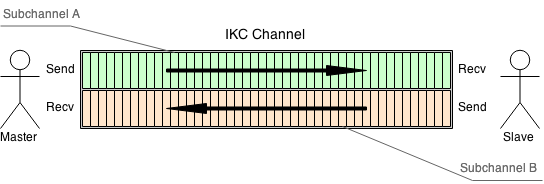
\includegraphics[width=\textwidth]{IKC_Structure.png}
		\caption{Inter-Kernel Communication Organization}
    		\label{fig:ikc}
	\end{figure} 
		
	There are three conceptual operations supported by channel:
	\begin{enumerate}
		\item Push. Paste the message specified into the first free space in the send subchannel. 
		\item Pop. Receives and removes the message from the recv subchannel.
		\item Peek. Receives but not removes message from the recv subchannel.
	\end{enumerate}
	
	Message size of the channel was chosen to be equal to 64 bytes. It was chosen that, because:
	\begin{enumerate}
		\item It is aligned to the cache line size. 
		Each message covers exactly two cache lines. 
		This property helps as to eliminate unwanted cache-line flip-flopping which reduce efficiency of communication. 
		\item It is a power of two. 
		That is mean that each subchannel contains 32 message slots which is also power of two. 
		This property allows us to easily and efficiently represent channel internally as a ring buffer.
		No one message can cross the border of the buffer, because channel size is divisible by message size and message size is fixed.
		We can use integer overflow safely for read and write pointers tracking, because overflow will occur only in places of going back to the first slot of buffer.
		All operation of multiplication, division and modulo operation will be optimized by compiler by bit shifting and masking, which will replace expensive (especially on ARM) arithmetical operations by simple and cheap analogs.
		If be honest we even not sure that ARM CPU used by Pandaboard provides hardware instructions for these operations or it relies on compiler which will implement them in software.
		In the same time we haven't checked that the expected behavior will be produced by compiler, because we haven't our binaries disassembled for explicit check (due to the lack of knowledge's of ARM assembler and appropriate disassembling software), but we sure that expected optimizations will be done, because it simple and well-known and this is exactly what we saw before for Microsoft Visual C++ compiler and IA-32 platform. 
		\item This message size allows to fit one native intra-kernel RPC message into one IKC message.
		\item Second cache line is almost unused for data transfer and last word of it used as a ready sign.
		This allows us to eliminate cache line flip-flopping between writer and reader, because while writer will fill first cache line of the message without any distortion reader will constantly check the last word of second cache line and also without any distortion. 
		When writer will have whole message flushed into channel, it will raise ready flag at the last word of second cache line of the message notifying reader that it can read the message safely now.
		As a result only three cache line passes between cores will occur: 2 line from reader to writer, 2 line from writer to reader and finally 1 line from writer to reader.  
	\end{enumerate}
	
	Each endpoint of the channel uses pair of channel pointers: read and write. 
	Read pointer if used for recv subchannel only and write pointer for send suchannel only.
	Note that the read and write pointer of the same subchannel will belong to different cores and will be tracked independently.
	They are not shared. 
	
\todo {}

- Spawning cores on low level.
- Setup of ELF image
- Communication between cores

\subsection{FAT file system}

The FAT filesystem is implemented in \filepath{aos\_support/fat32.c}, whereas the server and disk driver is located in \filepath{usr/mmchs/}.
We only support read operations on a FAT filesystem, and we didn't try to improve the block driver as well.

The main data structure for the FAT filesystem is the config struct:

\begin{lstlisting}
struct fat32_config {
    sector_read_function_t read_function;

    uint32_t volume_id_sector;
    uint32_t sectors_per_cluster;
    uint32_t fat_sector_begin;
    uint32_t cluster_sector_begin;
    uint32_t root_directory_cluster;
};
\end{lstlisting}

Within the struct we store some of the most important data, such as the start address of the File Allocation Table or the cluster region.
We also store a pointer to a function needed to read a block from disk.
That way we can easily reuse the FAT driver module for block devices other than the SD card of the Pandaboard.

A common operation in the FAT filesystem is to follow a chain of clusters and read consecutive sectors.
We added a small support structure \lstinline!struct sector_stream! to hide this complexity.
A sector stream is an iterator over a file or directory and can be advanced with \lstinline!stream_next!.

An important internal function is \lstinline!find_node!.
This function takes a path as an argument and tries to find a filesystem node (file or directory) with the given path.
If found it returns the start cluster and the file size (if it is a file) of the node.

\subsubsection{File management}

File operations are done in the usual open-read-close cycle and identified by a file descriptor.
When opening a file we call \lstinline!find_node! to search the filesystem for the file with the given path.
We then store a mapping from the file descriptor to the start cluster, the file size and the \lstinline!fat32_config!.

For file reads we use the \lstinline!sector_stream!.
We skip the first few sectors until we reach the position in the file requested by the user.
After that we just do a linear scan of the file and copy all bytes into a buffer.
To send the byte buffer back to the client we make use of the bulk transfer mechanism.

When closing a file we just discard the information collected during the open phase.

\subsubsection{Partition tables}

Due to the fact that Windows couldn't create an SD card without a partition table we had to add some rudimentary support for it.
The filesystem server loads the partition table and looks at the first partition table entry.
It then extracts the start block of the first partition and initializes the FAT driver with that information.

\subsubsection{Assessment}
\todo{Write assessment}

% - filesystem code in aos\_support/fat32.c
% - handler in mmchs/filesystem\_server.c
% - Currently read-only
% - some support for partition tables
% - Performance improvements: sequential read? cached FAT? bulk transfer?

\subsubsection{ ELF loading}

\todo {Implement ELF loading}

\section{Conclusion}

\begin{flushleft}
{{{
\bibliographystyle {plain}
\bibliography {./references}
}}}
\end{flushleft}


\todos

\end{document}          
 
